\chapter{Literature Review}\label{chap:review}
\section{Overview}
The research analyzes previous cryptanalysis work, including the design of block ciphers, cryptanalysis-related knowledge, including KATAN and Boomerang related literature needed for the research.


\section{Block ciphers and Cryptanalysis}\label{sec:symmetric_review}
This section describes the principle of symmetric-key encryption and introduces two symmetric-key ciphers. Then there is a review of cryptanalysis methods, and the details of these methods are described. This section provides help for understanding cryptanalysis.

\subsection{Block Cipher Designs}

Block cipher is an important part of symmetric-key encryption. The design concept of block cipher originated from \cite{6769090}. Its public research began with the publication of the DES algorithm \cite{pub1999data} in the late 1970s. The rapid development of block cipher theory and application Benefited from the AES \cite{dworkin2001advanced} program in the United States in the late 1990s  and the NESSIE program in Europe in the early 2000s. 

In the literature \cite{6769090}, from the perspective of resisting statistical attacks, Shannon proposed the ”confusion” and ”diffusion” criteria for designing encryption algorithms. Each element in the original text is rearranged in obfuscation, whereas in diffusion, each element is changed to be mapped to numerous elements in the ciphertext. This criterion is still one of the important principles to be followed in the design of block ciphers. In the AES plan and the NESSIE plan, the cryptography community has conducted extensive and in-depth research on the design and analysis theory of block ciphers, and the theory of block ciphers is perfect. In the SHA-3 project \cite{dworkin2015sha}, more than half of the Hash functions adopt the design concept of block ciphers, so block ciphers are becoming more and more important. 

The design of block ciphers usually follows the following two principles: the security principle and the implementation principle. The security principles include the principle of confusion, the principle of proliferation, and the principle of resistance to existing attacks. Implementation principles include software implementation principles and hardware implementation principles. Usually, the designed algorithm conforms to the above principles by iterative means: one method is to construct an iterative function with strong cryptographic properties, so that the number of iterations can be reduced; the other method is to construct an iterative function with relatively weak cryptographic properties, but The number of iterations is relatively high. In practical construction, the latter is usually adopted, that is, functions with weak cryptographic properties are iterated for many times to satisfy the security principle and the realization principle. 

The mathematic model of block cipher, $\mathbb{F}_2$ presents a binary field, $\mathbb{F}_2^n$ and $\mathbb{F}_2^m$ present $n$ and $m$ dimensional vector spaces, respectively. $S_K\in \mathbb{F}_2^m$ is a key space, then the ciphers can present two reflections.

\begin{equation}
    \begin{aligned}
        E: F_2^n \times S_k \to F_2^n,\\
        D: F_2^n \times S_k \to F_2^n.
    \end{aligned}
\end{equation}


The basic structure of commonly used block ciphers will be described below.

\subsubsection{Feistel Structure}
The IBM researchers that developed the DES algorithm also came up with the Feistel structure, which eventually gained popularity. Referring to Figure \ref{fig:Feistel}, the encryption procedure for the r-round Feistel structure cipher with a $2n$ block length is as follows: Given a civilization $P$ with $2n$ bits, divide it into two left and right n bits, where $L_0$ is the left $n$ bits and $R_0$ is the right $n$ bits, and then, in accordance with \eqref{eq:Feistel}, repeat the procedure $r$ times.

\begin{equation}
    \begin{aligned}
        \begin{cases}
            L_i = R_{i-1}\\
            R_i=L_{i-1}\oplus F(R_{i-1},K_i)
        \end{cases}
    \end{aligned}  
    i=1,2,\dots,r  
    \label{eq:Feistel}
\end{equation}

Here, $\oplus$ denotes an XOR operation, $F: \mathbb{F}^n_2\times \mathbb{F}^m_2\to \mathbb{F}^n_2$ stands for "round," and $K_1,K_2,\dots, K_r$ According to the key expansion method, $K_r$ is the round key produced by the seed key $K$, and $m$ is the round key's length. The final round typically does not require "left and right exchange," meaning that the ciphertext is $C=R_rL_r$. The slower diffusion effect is a drawback of Feistel.


\begin{figure}[hbt!]
    \centering
    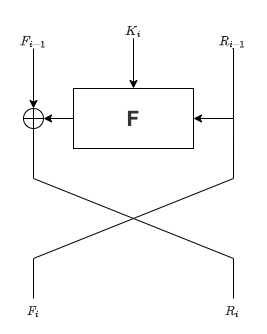
\includegraphics[width=45mm]{Feistel}
    \caption[Boomerang Attack Model]{Feistel Structure}\label{fig:Feistel}
\end{figure}

\subsubsection{SPN Structure}
A reversible linear transformation P and a reversible nonlinear function S, controlled by a round key, typically make up each round of the SPN structure. The S-transform layer serves as the obfuscation layer in this construction, and the P-transform layer serves as the diffusion layer. The SPN structure has a faster diffusion effect than the Feistel structure, and the designer can use this structure to provide algorithms resistant to differential cryptanalysis and linear ciphers with a provable security for analysis.
\begin{equation}
    \begin{aligned}
        \begin{cases}
            Y&=S(X_{i-1},K_i)\\
            X_i&=P(Y)
        \end{cases}
    \end{aligned}
    i=1,2,\dots,r  
    \label{eq2}
\end{equation}
The encryption procedure for the r-round SPN structure cipher with an n-block length is as follows: Let $P=X_0$, where $P$ is the plaintext with $n$ bits, and follow \eqref{eq2} to carry out the same procedure for $r$ rounds.

In SPN structured ciphers, the last round of $P$ transformation is usually replaced by key addition.

\begin{figure}[hbt!]
    \centering
    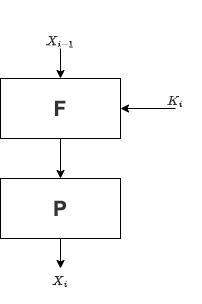
\includegraphics[width=45mm]{SPN}
    \caption[Boomerang Attack Model]{SPN Structure}\label{fig:SPN}
\end{figure}

\subsubsection{Lai-Massey Structure}
When developing the IDEA algorithm, Lai and Massey proposed a framework they called the Lai-Massey structure. Most of the time, the Lai-Massey structure has the benefit of consistent encryption and decryption.

\begin{figure}[hbt!]
    \centering
    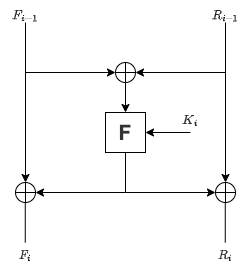
\includegraphics[width=45mm]{Lai_Massey.png}
    \caption[Boomerang Attack Model]{Lai-Massey Structure}\label{fig:Lai_Massey}
\end{figure}

For the r-round Lai-Massey structure cipher with a block length of 2n, the encryption process is as follows: Given a 2n-bit plaintext $P$, first divide it into two n-bit parts on the left and right, and denote $L_0$ as the left $n$ bits of $P$, and $R_0$ as the right $n$ bits of $P$, then $P=L_0R_0$. Then according to \eqref{eq3}, $r$ rounds of exactly the same operations are performed.

\begin{equation}
    \begin{aligned}
        \begin{cases}
            T&=F(L_{i-1}\oplus R_{i-1},K_i)\\
            L_i&=L_{i-1}\oplus T\\
            R_i&=R_{i-1}\oplus T
        \end{cases}
    \end{aligned}
    i=1,2,\dots,r  
    \label{eq3}
\end{equation}

\subsubsection{Summary}
The overall structure is an important feature of block cipher algorithms. Different structures have a great impact on the selection of the round function and the performance on various platforms. In addition to the above three mainstream structures, the overall structure also includes generalized (non-)equilibrium Feistel structure, MISTY structure and the mixed use of various structures. In addition, the round functions of many cryptographic algorithms adopt different structures. For example, the Camellia algorithm adopts the Feistel structure as a whole, but the round function adopts the SPN structure; the FOX algorithm adopts the Lai-Massey structure as a whole, and the round function adopts the SPS structure. The structure used to design an algorithm mainly depends on the performance requirements of the algorithm, the construction of sub-modules, and the security of the overall structure.


\subsection{KATAN family cipher}
KATAN family cipher is a hardware oriented block ciphers and was proposed in CHES 2009 \cite{10.1007/978-3-642-04138-9_20}. KATAN family has three variants of KATAN are KATAN32, KATAN48 and KATAN64. Each various contains six block ciphers divide into two flavors, in the first flavor is composed of three block ciphers, with 32,48 or 64 bit block size, and in the second flavor contains the other three ciphers with same block size. They are use 80-bit key size. KATAN use an extending key algorithm to make 80-bit key to 508bit sub-key. Suppose a key $k$ is 80-bit, and $k_i$ present i-th bit in $K$, the sub-key is given by:
\begin{equation}
    sk_i=
\left\{
    \begin{aligned}
        &k_i\qquad\qquad\qquad for\quad i = 0\dots 79\\
        &k_{i-80}\oplus k_{i-61}\oplus k_{i-50}\oplus k_{i-13}\quad Otherwise
    \end{aligned}
\right.
\end{equation}The round function of KATAN, the plaintext be divided two part and be loaded to two register $L_1$ and $L_2$, then the update processes are shown as follows:
\begin{equation}
    \begin{aligned}
        f_a(L_1) &= L_1[x_1]\oplus L_1[x_2]\oplus (L_1[x_3])\cdot L_1[x_4])\oplus(L_1[x_5]\cdot IR)\oplus k_a\\
    f_b(L_2) &= L_2[y_1]\oplus L_2[y_2]\oplus (L_2[y_3])\cdot L_2[y_4])\oplus(L_2[y_5]\cdot L_2[y_6])\oplus k_b\\
    L_1[i] &= L_1[i-1](i\leq i\le |L_1|), L_1[0]=f_b(L_2),\\
    L_2[i]&=L_2[i-1](i\leq i\le |L_2|), L_2[0]=f_b(L_1),\\    
    \end{aligned}
\end{equation}
 where $\oplus$ and $\cdot$ are bitwise $XOR$ and $AND$ operations, respectively, and $L[x]$ denotes the x\-th bit of $L$, $IR$ is the round constant value defined in the specification, and ka and kb are two subkey bits. For round $i$, $k_a$ and $k_b$ correspond to $sk_{2(i-1)}$ and $sk_{2(i-1)+1}$. The parameters of KATAN family are shown in TABLE \ref{tb:KATAN_P}.
 \begin{table}[htbp]
	\centering  
	\caption{Parameters of KATAN family} 
	\label{tb:KATAN_P} 
	\begin{tabular}{|c||c|c|c|c|c|c|c|c|c|c|c|c|c|c|c|c|}  
        \hline  
        algorithm&|$L_1$|&|$L_2$|&$x_1$&$x_2$&$x_3$&$x_4$&$x_5$&$y_1$&$y_2$&$y_3$&$y_4$&$y_5$&$y_6$\\
		\hline  
		KATAN32&13&19&12&7&8&5&3&18&7&12&10&8&3\\
        KATAN48&19&29&18&12&15&7&6&28&19&21&13&15&6\\
        KATAN64&25&39&24&15&20&11&9&38&25&33&21&14&9\\
		\hline
	\end{tabular}
\end{table}






\subsection{Cryptanalysis}
There are two basic ways to measure the security of a cryptographic algorithm: one is actual security, and the other is unconditional security (theoretical security). The actual security is evaluated according to the amount of computation required to decipher the cryptosystem. For example, the security of the RSA system is based on the difficulty of decomposing large integers, but with the development of computer technology, RSA may also be vulnerable. Theoretical security is independent of an adversary's computing power and time, and any effort to decipher an algorithm will be no better than random selection. 

Most of the cryptanalysis methods proposed in the papers follow Kerckhoffs's principle: The principle holds that a cryptosystem should be secure, even if everything about the system, except the key, is public knowledge. According to the Kerckhoffs's principle, the security of a cryptographic algorithm should depend on the secrecy of the key, not the secrecy of the algorithm itself.

Many literatures propose different cryptanalysis methods to analyze the target algorithms they specify. What is important is whether these algorithms have extremely high accuracy, whether they undermine practical security or theoretical security, in which threats to practical security are very serious issues. In the following, we provide an overview of the cryptanalysis of block ciphers.

The method of cryptanalysis is divided into brute force attack, the security of the algorithm is studied based on the mathematical method, and the security of the algorithm and the security of the algorithm under different usage modes are studied in combination with the physical realization method. 

According to the different environments, password attacks can be divided into the following four types:
\begin{itemize}
    \item Ciphertext-only attack: A cryptanalyst has one or more ciphertexts encrypted with the same key, and analyzes these decrypted ciphertexts to obtain the plaintext or key.
    \item Known-Plaintext Attack: A cryptanalyst has some plaintexts and ciphertexts of these plaintexts encrypted with the same key, and recovers the key by analyzing these known plaintexts and the corresponding ciphertexts.
    \item Chosen-plaintext attack: The cryptanalyst can choose the plaintext he wants at will and encrypt it, and recover the key according to the selected plaintext and the corresponding ciphertext.
    \item Chosen ciphertext attack: The cryptanalyst can freely select the ciphertext he wants and decrypt it, and recover the key according to the chosen ciphertext and the corresponding plaintext.
\end{itemize}Then, the research on analytical ciphers is usually based on three different foundations.

\subsubsection{Brute-force}
Brute-force attacks are the simplest and least effective, they generally include four methods:\begin{itemize}
    \item Exhaustive key search: Under a ciphertext-only attack, the attacker uses all possible keys to continue decrypting one or more ciphertexts until a meaningful plaintext is obtained. This method can decipher any block cipher in theory, but its efficiency is the lowest. In practical cryptanalysis, it is usually used in combination with other analysis methods.
    \item Dictionary attack: The attacker collects pairs of plaintext and ciphertext and arranges them into a "dictionary". When seeing a ciphertext, the attacker checks whether it exists in the dictionary, and if so, finds the corresponding plaintext.
    \item Table lookup attack: This method is a chosen plaintext attack. The attacker uses all possible keys to encrypt the same plaintext, and stores the key and the corresponding ciphertext. When obtaining the plaintext and ciphertext, the attacker only needs to Find the corresponding key in the storage table.
    \item Time-tradeoff attack: This is a chosen-plaintext attack method, proposed by Hellmma, by using a combination of exhaustive key search and table lookup attack.
\end{itemize}Although these methods are not very useful in practice, the complexity of exhaustive key search is used as an indicator to measure the efficiency of an attacking algorithm. 

\subsubsection{Based on the Security of Algorithms Based on Mathematical Methods}
This method mainly includes two aspects: one is to study how to distinguish cryptographic algorithms from random permutation. In cryptanalysis, for the same indicator, first calculate its value under random permutation, and then calculate the corresponding value of a cryptographic algorithm in a certain cryptographic algorithm. If the two values are significantly different, then this metric can distinguish a cryptographic algorithm from random permutation. In cryptanalysis, if for some specific form of plaintext input, the corresponding ciphertext follows a special rule, it is said to find an effective distinguisher of the algorithm. The second is to study how to obtain the key information of the cryptographic algorithm. For iterative block ciphers, the cryptanalyst first finds an efficient distinguisher of the reduced-rounds algorithm, and then verifies the correctness of the distinguisher by guessing some of the round keys. When an effective distinguisher of the cryptographic algorithm is found, there are usually two ways to recover the secret: one is the statistical method, for the guess value of each key, according to certain rules (usually related to the distinguisher) collected plain ciphertext Statistical analysis is performed, and the final value with a clear statistical advantage may be the correct key. The another is to solve by algebraic method. In this method, the transformation corresponding to encryption and decryption is represented by a system of equations. Through certain mathematical methods, the root of the system of equations is solved to obtain the key information. Common math-based methods include:
\begin{itemize}
    \item differential cryptanalysis
    \item linear cryptanalysis
    \item meet-in-the-middle attack
    \item collision attack 
    \item Square attack 
    \item interpolation attack
    \item correlated key attack 
    \item boomerang attack
\end{itemize}
With the development of cryptanalysis, more methods have been proposed.

\subsubsection{The security of algorithms is related to they way it is implemented in hardware}
In the traditional research on the security of algorithms based on mathematical methods, the encryption or decryption process of the algorithm is generally regarded as a transformation with secret parameters, and the key information is inferred only by obtaining the input and output of the transformation. At the end of the 20th century, a new attack method appeared in the cryptography world. In addition to the traditional mathematical method, this attack method also combines the information differences represented by certain physical parameters such as time, energy, electromagnetic, temperature, sound, etc. to infer information about the key. This attack method combined with physical implementation is generally called side channel attack. At present, common side-channel attacks mainly include timing attacks, energy analysis, fault attacks, electromagnetic attacks, and cache attacks.

\section{Cryptanalysis Method}\label{cry_method}
This section describes details of several attacks.

\subsection{Differential Attack}
The differential attack is one most effective methods to attack iterative block ciphers,  and it is an important index for evaluating the security of block ciphers. \cite{biham1991differential} proposed this analysis method. It finds the difference between specific pairs of plaintext and ciphertext to distinguish block ciphers from random permutations and then recovers the key. 

We assume a block cipher, $E\{0,1\}^n \times \{0,1\}^l \to \{0,1\}^n$, and $n, l$ present length of a block and length of the key, respectively. For $k \in \{0,1\}^l$, the permutation be presented $E_k(\cdot)=E(\cdot, k)$ on $\{0,1\}^n$. The encryption function $E_k(\cdot)$ is consist of $r$ sub\-encryption functions which use sub-key $k_i, i=1,2,3,4…,r$ to encrypt. The encyrption equation as \ref{block_cipher_eq}.

\begin{equation}
    \label{block_cipher_eq}
    E_k(x)=F_{k_r}\circ F_{k_{r-1}}\circ \dots \circ F_{k_2}\circ F_{k_1}(x).
\end{equation}
Next, $Y_{i-1}, Y_i$ present the input and output on i-th round, in other words, $Y_i=F_{k_i}(Y_{i-1})$. $X,Z=Y_r$ present the input(plaintext) of the first round and the output of the last round, respectively. There are three important definitions. First, \textbf{Difference}, the difference of $X, X^*\in\{0,1\}^n$ is $\Delta X = X\oplus X^*$. Second, \textbf{Differential}, presents a propagation from difference $\alpha$ to difference $\beta$.
Last, \textbf{Differential characteristic}, a differential characteristic of $i$ rounds, $\Omega = (\beta_0,\beta_1\dots,\beta_{i-1},\beta_i)$ when the difference of the input pairs $(X,X^*)$ satisfy $X\oplus X^*=\beta_0$, and in i-th round, the middle states $(Y_j ,Y_j^*)$ satisfy $Y_j\oplus Y_j^*=\beta_j$. The equation \ref{eq:DP_alpha_beta} presents the probability of a differential,
\begin{equation}
    \label{eq:DP_alpha_beta}
DP(\alpha,\beta) = \underset{X,K}{Prob}\{F(X,K)\oplus F(X\oplus \alpha, K)=\beta\},
\end{equation} when the number of rounds more than 1 can derive the probability of a differential characteristic $\Omega = (\beta_0, \beta_1,\dots,\beta_i)$ in following.
\begin{equation}
DP(\Omega)=\prod_{j=1}^iDP(\beta_{j-1}, \beta_j).
\end{equation}
In Feistel or SPN structure ciphers, the S-box is the only nonlinear part of the round function, so we need to make \textbf{Differential Distributed Table(DDT)} if we want to find a differential path with high probability. There is an example of DDT of present cipher is Figure \ref{fig:ddt}. The first row present difference of out, and first column present difference of input to S-BOX. Suppose $S:\{0,1\}^n\to\{0,1\}^n$ an n-bit to n-bit S-BOX,the element of DDT is given by:
\begin{equation}
    (\Delta_{in}, \Delta_{out})=\#\{P_i\oplus P_i^*=\Delta_{in}|S(P_i)\oplus S(P_i^*)=\Delta_{out}\}
\end{equation}
\begin{figure}[hbt!]
    \centering
    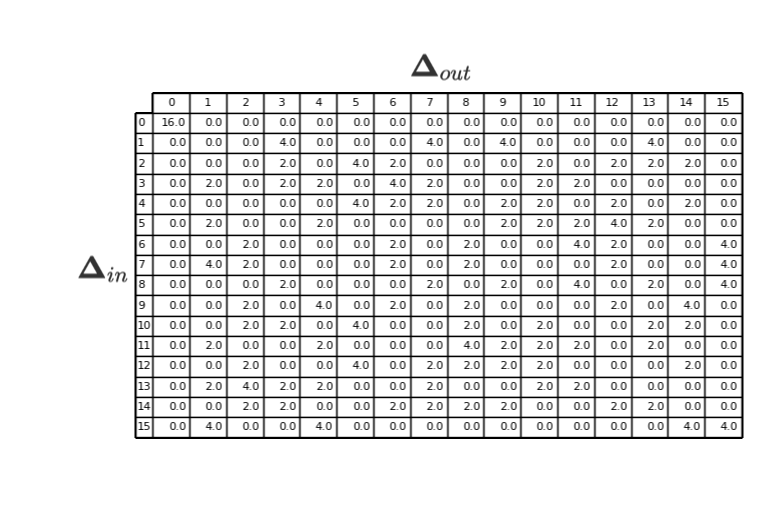
\includegraphics[width=100mm]{DDT.png}
    \caption[Differential Distributed Table]{Differential Distributed Table}\label{fig:ddt}
\end{figure}
The probability of a pair($\Delta_{in}, \Delta_{out}$) is $p=\frac{pos(\Delta_{in}, \Delta_{out})}{2^n}$. The differential attack steps are summarized as follows:
\begin{enumerate}
    \item To find a high probability differential characteristic of $r-1$ rounds, the probability is presented as $p$.
    \item To determine the sub-key in the i-th round by the output of the differential characteristic. Assume the length of the key attacked is $l$ bits, to set $2^l$ counters, each counter corresponding to each possible candidate key.
    \item Generate the plaintext  $X$ uniformly at random, $X^*$ satisfy $X^*=X\oplus \alpha$. To encrypt $X, X^*$ to get ciphertexts $Z, Z^*$, respectively. The number of generated plaintext pairs is $m \approx c \times \frac{1}{p}$, $c$ presents a constant number.
    \item For each ciphertext pairs, use candidate sub-key to decrypt $Z, Z^*$, the difference of the decrypted data $\Delta = F^{-1}_{gk_i}\oplus F^{-1}_{gk_i}(Z^*)$, if $\Delta = \beta$, then the counter corresponding to the candidate key is plus 1.
    \item The max value of these counter corresponding to the candidate key is correct sub-key.
\end{enumerate}

\subsection{Linear Cryptanalysis}
A Japanese researcher \cite{matsui1993linear} proposed a new cryptanalysis method in Eurocrypt 1993. The same year, in Crypto 1993, he published new two linear approximation relations, and he use these relations to crack DES, using 12 workshops and 50 days. There are results of the first experimental analysis of DES in the open literature. Unlike differential cryptanalysis, linear cryptanalysis is a known-plaintext attack method. It distinguishes block ciphers and random permutations by finding effective linear approximation relations between plaintext and ciphertext and recovers the key. Remember a block cipher defined in \ref{block_cipher_eq}. In linear cryptanalysis, assume $a,b\in \{0,1\}^n$ and $a=(a_1,a_2,a_3,…,a_n), b=(b_1,b_2,…,b_n)$, $F(x,k)$ presents the round function,  given two linear mask $(\alpha,\beta)$, the linear expression approximation formula is
\begin{equation}
\alpha \cdot x \oplus \beta \cdot F(x,k).
\end{equation} 
In this formula, $\cdot$ present multiplication in a binary field. Assume $p$ presents the probability of the linear expression approximation formula of $\alpha$ and $\beta$, then the linear probability can present these:
\begin{equation}
\begin{aligned}
Bias: \zeta_F &= p(\alpha,\beta) - \frac{1}{2},\\
Correlation: Cor_F &= 2p(\alpha, \beta) -1,\\
Potential: Pot_F &= (p(\alpha, \beta)-\frac{1}{2})^2.
\end{aligned}
\end{equation}. In paper [28,39], if the define the linear expression approximation formula of  linear mask $(\alpha,\beta)$ is
\begin{equation}
LP(\alpha,\beta) = (2\cdot \underset{X,K}{Prob}\{\alpha \cdot X=\beta \cdot F(X,K)\}-1)^2
\end{equation}, the $LP$ can corresponding to $DP$ of differential cryptanalysis. The steps of linear cryptanalysis as follows:
\begin{enumerate}
    \item To find r-1 rounds differential approximation formula that bias $zeta(\alpha, \beta)$ relatively large.
    \item To determine the sub-key in the i-th round by the output of the differential characteristic. Assume the length of the key attacked is $l$ bits, to set $2^l$ counters, each counter corresponding to each possible candidate key.
    \item Select the plaintext $X$ uniformly at random. To encrypt $X$ to get ciphertext $Z$, respectively. The number of generated plaintext pairs is $m \approx c \times \frac{1}{\zeta^2}$, $c$ presents a constant number.
    \item For each ciphertext $Z$, decrypt it to get $Y_{r-1}$ using candidate sub-keys, if $\alpha x\cdot X\oplus \beta \cdot Y_{r-1}=0$, then the corresponding counter is plus 1.
    \item The max value of $|\frac{\lambda^i}{m}-\frac{1}{2}|$ of these counter corresponding to the candidate key is correct sub-key.
\end{enumerate}

\subsection{Boomerang Attack}
The boomerang attack is a differential-style attack, it can find a higher probability of differential characteristics than a differential attack and it is a more effective cryptanalysis method of block ciphers. \cite{10.1007/3-540-48519-8_12} proposed this attack upon discovering good differential characteristics for the first four and last four Feistel rounds of COCONUT98. The boomerang attack has more power when it combined with other cryptanalysis method, it has been demonstrated when it is used to break the full-round AES-192/256 \cite{biryukov2009related} and the full-round KASUMI \cite{biham2005related} in the related-key setting.


Figure \ref{fig:boomerang} shows the structure of the boomerang attack. Four plaintexts $P_1$, $P_2$, $P_3$, $P_4$ and with their respective ciphertexts $C_0$, $C_1$, $C_2$, $C_3$; The $E(\cdot)$ present the encryption operation and decompose the cipher into $E=E_0 \circ E_1$ where $E_0$ represent the first half of the cipher and $E_1$ presents last half. There are four differential trails, $\alpha\to \beta$ for $E_0$; $r\to\delta$ for $E_1$; $\delta \to r$ for $E_1^{-1}$ and $\beta\to\alpha$ for $E_0^{-1}$.

The pair $P_0$ and $P_1$ with the trail for $E_0$ and the pairs $P_0,P_2$ and $P_1,P_3$ satisfy the trails for $E_1^{-1}$, then the pair $P_2$, $P_3$ is set up to use the trail $\beta\to\alpha$ for $E_0^{-1}$. Consider the intermediate value after half of the rounds, when the previous three trails hold, the formula \ref{boomerang_1} tell why.

\begin{equation}
    \begin{aligned}
        \label{boomerang_1}
        E_0(P_2)\oplus E_0(P_3)&=E_0(P_0)\oplus E_0(P_1)\oplus E_0(P_0)\oplus E_0(P_2) \oplus E_0(P_1) \oplus E_0(P_3)\\
        &=E_0(P)\oplus E_0(P_1)\oplus E_1^{-1}(C_0)\oplus E_1^{-1}(C_2)\oplus E_1^{-1}(C_1)\oplus E_1^{-1}(C_3)\\
        &=\beta \oplus r \oplus r\\
        &=\beta
    \end{aligned}
\end{equation}
Because the other three differential trails are holding, when the equation is satisfied, a pair of plaintexts $P_2,P_3$ has the same difference as found in original plaintexts. The idea of boomerang attack is to use such quartet of plaintext and of ciphertext to find key information, and use the information to recover key. In section 4 of \cite{10.1007/3-540-48519-8_12} states that probability of a quartet, assume $p_0$ is the probability of the differential trail $\alpha\to\beta$ for $E_0$ and $p_1$ is the probability of the differential trail $\delta\to r$ for $E_1$. Then the probability $p$ of a right quartet satisfy
\begin{equation}
    p\ge p_0^2p_1^2.
\end{equation}

The boomerang attack has some variants, such as amplified boomerang analysis \cite{kelsey2000amplified} and rectangle analysis \cite{biham2001rectangle}. In recent years, a new cryptanalysis method \cite{dunkelman2020retracing} based on this idea has been proposed, called the retracing boomerang attack , this new attack reduces the complexity of the boomerang method to analyse AES(5-ROUNDS) from $2^{24}$ to $2^{16.5}$. Also, the boomerang attack can achieve more efficiency with other cryptanalysis methods, such as the related-key method. In \cite{inproceedings}, the boomerang attack with a related-key setting achieves the best result for the boomerang to analyse KATAN48/64. But \cite{5730575} published results of several experiments, to demonstrate the boomerang analysis can commonly give highly inaccurate probability values and he shows the boomerang attack is used to analyse DES and AES on some parameters, then the boomerang never comes back.

For the problem, \cite{10.1007/978-3-319-78375-8_22} gives a solution. It proposed new tools to improve the reliability of the sandwich attack, called Boomerang Connectivity Table(BTC). The sandwich attack is a boomerang-style attack depicted in Fig \ref{fig:sandwich}, it defines $E=E_1\cdot E_m\cdot E_0$ where $E_m$ is a relatively short operation satisfying some differential propagation among four texts with probability $r$, then the entire probability is $p^2q^2r$. \cite{dunkelman2010practical} define r as follows.
\begin{equation}
    r=Pr[(x_3\oplus x_4)=\beta|(x_1\oplus x_2=\beta)\wedge (y_1\oplus y_3=r)\wedge(y_2\oplus y_4)=r]
    \label{r_prob}
\end{equation}
The BTC can evaluate $r$ in efficacy and easy-to-understand way when $E_m$ is composed of a single S-BOX layer. In this situation, for a given pair of ($\Delta_i, \bigtriangledown_o$), the probability that a right quartet is generated in each S-BOX in the middle S-BOX layer is given by:
\begin{equation}
\frac{\#\{x\in{0,1}^n|S^{-1}(S(x)\oplus \bigtriangledown_o)\oplus S^{-1}(S(x\oplus \Delta_i)\oplus \bigtriangledown_o)=\Delta_i\}}{2^n}
\label{btc_p}
\end{equation}
Where $S:\{0,1\}^n\to \{0,1\}^n$ is an n-bit to n-bit S-box and $S^{-1}$ is its inverse. When $E_m$ is a single S-BOX layer, the result of Equation\ref{btc_p} is exactly r in Equation\ref{r_prob}. \cite{10.1007/978-3-319-78375-8_22} demonstrate that the result of using BTC is more than the result only using DDT.
\begin{figure}[hbt!]
    \centering
    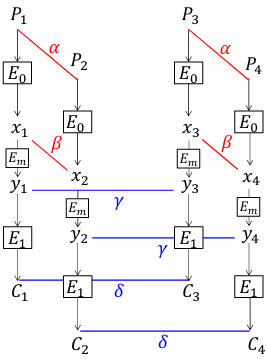
\includegraphics[width=45mm]{sandwich.png}
    \caption[Boomerang Attack Model]{Sandwich Attack Model}\label{fig:sandwich}
    \end{figure}

The BTC is not a panacea and can only use ciphers based on S-BOX in practice so far. There is discuss BTC use to ciphers based on ARX in \cite{10.1007/978-3-319-78375-8_22}, also points out S-BOX swich not work in ARX.

\section{Chapter Summary}\label{sec:lit_summary}

Section \ref{sec:symmetric_review} discussed the design of block ciphers and introduces three types of design structures, then introduces the basic theory of cryptanalysis and the design of KATAN. Section \ref{cry_method} describe the detail of the differential attack, the linear attack and boomerang attack, and discuss the advantages and disadvantages of BTC, this contents of this section are closely related to this study.